\section{Хэрэглэгчийн шаардлага} 

\subsection{Хэрэглэгчид болон түүний эрх} 
\begin{itemize}
	\item Хилээр нэвтэрж буй зорчигч
	\begin{itemize}
	    \item ХШ110. Системд бүртгүүлэх  
	    \item ХШ120. Системд нэвтрэх 
	    \item ХШ130. Бичиг баримт баталгаажуулах 
            \item ХШ140. Хувийн мэдээлэл засварлах 
            \item ХШ150. Асуулга бөглөх
            \item ХШ160. Асуулга засварлах 
            \item ХШ170. Вакцины гэрчилгээ оруулах
            \item ХШ180. Автомашинаар зорчиж буй тохиолдолд дугаар оруулах. 
	\end{itemize}

        \item Гаалийн Хорио Цээрийн газрын Ахлах байцаагч
	\begin{itemize}
	    \item ХШ200. Асуумж захиран зохицуулах
                \begin{itemize}
                    \item ХШ201. Асуулт нэмэх
                    \item ХШ202. Асуулт засварлах
                    \item ХШ201. Асуулт устгах
                    \item ХШ201. Асуултуудын дараалал солих
                \end{itemize}
	    \item ХШ210. Асуумжийн тайлан хянах
                \item ХШ211. Тайлан асуултын хариултаар шүүх 
                \item ХШ211. Тайлан хэрэглэгчийн мэдээллээр шүүх 
	\end{itemize}
        
	\item Ээлжийн ахлах
	\begin{itemize}
	    \item ХШ300. Нислэгийн мэдээлэл захиран зохицуулах 
            \begin{itemize}
                \item ХШ301. Нислэгийн мэдээлэл бүртгэх 
                \item ХШ302. Нислэгийн мэдээлэл засварлах 
                \item ХШ303. Нислэгийн мэдээлэл устгах 
            \end{itemize}
            \item ХШ310. Боомтын мэдээлэл захиран зохицуулах 
            \begin{itemize}
                \item ХШ311. Боомтын мэдээлэл бүртгэх 
                \item ХШ312. Боомтын мэдээлэл засварлах 
                \item ХШ313. Боомтын мэдээлэл устгах 
            \end{itemize}
	\end{itemize}

        \begin{itemize}
            \item ХШ400. Зорчигчийн халуун хэмжилтийн үр дүн оруулах
        \end{itemize}
\end{itemize}

\subsection{Функционал шаардлагууд}
\begin{itemize}
    \item Зорчигчийн харьцах хэсгийн функциональ шаардлагууд 
    \begin{itemize}
        \item ЗФШ100. Монгол хэрэглэгчийн регистерийн дугаараар хувийн мэдээлэл татдаг байх
        \item ЗФШ200. Зорчигчийн нэвтрэх нэр давхардуулахгүй байх 
        \item ЗФШ300. Зорчигчийн нууц үгийг хадгалахдаа буцаан задлах боломжгүйгээр нууцлах
        \item ЗФШ400. Зорчигч нэвтрэх нэр, нууц үг засварлах боломжтой байх 
        \item ЗФШ500. Зорчигч асуумжийг дутуу бөглөхөд анхааруулга өгдөг байх  
    \end{itemize}

    \item Хяналтын хэсгийн функциональ шаардлагууд 
    \begin{itemize}
        \item ХФШ100. Асуумжийн сэжигтэй тохиолдлуудыг ялган харуулдаг байх
        \item ХФШ200. Тайланг хариултаар нь шүүх боломжтой байх
        \item ХФШ300. Зорчигчийн бөглөсөн асуумжийн хариултуудыг QR code-оор дэлгэрэнгүй харах боломжтой байх
        \item ХФШ400. Асуултын шинэ эрэмбийг оруулахад бусад асуултын эрэмбийг харьцангуйгаар өөрчлөх 
        \item ХФШ500. Халдварын мутацлагдсан хэлбэр илэрсэн улсыг тодруулан харуулдаг байх 
        \item ХФШ600. Зорчигч болон байцаагчийн мэдээллийг регистерийн дугаар болон нэрээр нь хайх
    \end{itemize}

    \item Системийн функциональ шаардлагууд
    \begin{itemize}
        \item СФШ100. Хур системээс мэдээлэл татахдаа хэрэглэгчийн мэдээлэл нууцлах
        \item СФШ200. Хур системээс мэдээлэл татахдаа XML формат JSON формат хооронд шилжүүлэх
        \item СФШ300. Их хэмжээний өгөгдлөлийг хэсэгчлэн авах боломжтой байх
        \item СФШ400. Монгол, Англи, Орос, Хятад, Солонгос хэл дээр орчуулах боломжтой байх
        \item СФШ500. Файл хадгалах 
        \item СФШ600. Файл хадгалахдаа төрлийг нь тодорхойлон зураг болон баримт үед л хадгалах 
        \item СФШ700. Асуумж бөглөх хэсэгт оролтын утга нь ямар байхыг өгөгдлийн сан дээрх формат ашиглан шалгах, буруу үед мэдэгдэл өгөх. 
        \item СФШ800. Систем нь мэдэгдэл өгдөг байх. 
        \item СФШ900. Зорчигчийн мейл хаяг болон утасны дугаар луу OTP code илгээх
        \item СФШ1000. Нэвтэрсэн хэрэглэгчид token үүсгэж баталгаажуулалтад шаардлагатай үйл ажиллагаа бүрт token шалгах. 
        \item СФШ1100. Хяналтын харьцах хэсэг дээрх байгууллагатай холбоотой мэдээллийг засварлах эрхтэй эсэхийг тухайн байгууллагад бүртгэлтэй эсэхийг шалгах
        \item СФШ1200. Хяналтын харьцах хэсэг дээрх мэдээллийг хэрэглэгч засварлах эрхтэй эсэхийг харгалзах үйл ажиллагаа тухайн хэрэглэгчийн хувьд зөвшөөрөгдсөн эсэхийг шалгах. 
        \item СФШ1300. Олон боомтод ажилладаг байцаагчийн хувьд нэг бүртгэл үүсгэн байгууллагын эрхийг солих боломжтой байх. 
    \end{itemize}
\end{itemize}

\subsection{Функциональ бус шаардлагууд}
\begin{itemize}
    \item Аюулгүй байдал 
    \begin{itemize}
        \item ФБШ100. Хэрэглэгчийн нууц үгийг хадгалахдаа hash функц ашиглах ба буцаан анхны утгыг авах боломжгүй байна. 
        \item ФБШ200. Хур систем рүү хүсэлт илгээхдээ хэрэглэгчийн мэдээллийг RSA нууцлал ашиглан encrypt хийх. 
        \item ФБШ300. Хяналтын систем дээрх үйлдэл бүрийг хэрэглэгчийн эрхээр тохируулах ба хэрэглэгч бүр нь өөрийн эрхэд үл харгалзах үйлдлийг хийх боломжгүй байна. 
        \item ФБШ400. Баталгаажуулалт шаардлагатай үйлдэл бүрт token шалган тухайн хэрэглэгчийн бүртгэлийг баталгаажуулах 
    \end{itemize}

    \item Хүртээмжтэй байдал 
    \begin{itemize}
        \item ФБШ500. Систем нь унасан тохиолдолд шууд сэргэх боломжтой байх. 
        \item ФБШ600. Алдааны мэдэгдэлийг хэрэглэгчид ойлгомжтой байхаар илгээх 
        \item ФБШ700. Хянах хэсэг дээрх тайланг excel файл болгон импортлох боломжтой байх. 
    \end{itemize}

    \item Гүйцэтгэл 
    \begin{itemize}
        \item ФБШ700. Аливаа хүсэлтийг 2 секундийн дотор боловсруулдаг байх
    \end{itemize}
\end{itemize}

\section{USE CASE DIAGRAM}
\begin{figure}[H]
    \centering
    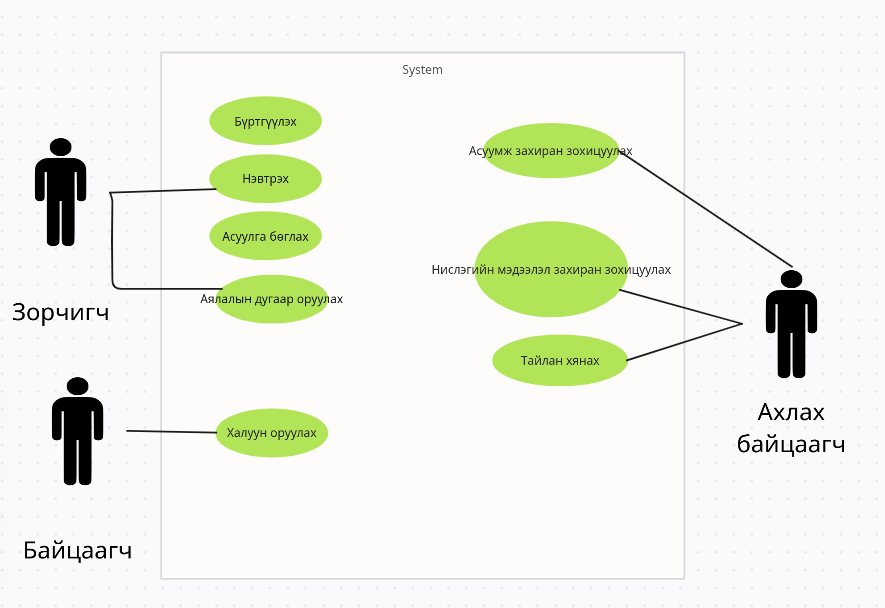
\includegraphics[scale=0.5]{usecase.png}
    \caption{Use Case Diagram}
    \label{fig:my_label}
\end{figure}
